%folders not useful = html images
\documentclass{article}
\usepackage{palatino,a4wide,epsfig}
\title{Programmers Guide to MusicLib}
\author{Daniel Bakker}

\begin{document}
\maketitle
\newpage
\tableofcontents
\newpage
\section{Overview}
This document describes the different sections of the MusicLib program and the functionality of each file included within it. This guide is designed for programmers interested in examining or modifying the source code. Reading the code itself will explain much more of the details, this guide is designed to point out which code to read.

Analysis and requirements specifications for this project can be found at;

``http://www.cosc.canterbury.ac.nz/teaching/handouts/cosc204/casestudy\verb|_|2.pdf''.


The MusicLib program is divided up into two main layers;
\begin{description} 
\item[The Database Layer] controls all the storing and recovering of information received from users.
\item[The CGI Layer] controls the web interface and generation of the html pages.
\end{description}

Some files are used by both the Database and the CGI layer, these are located in the directory named ``shared''.

All the web pages are Xhtml 1.0 compliant visit ``http://w3.org'' for more details.
\begin{figure}
\begin{center}
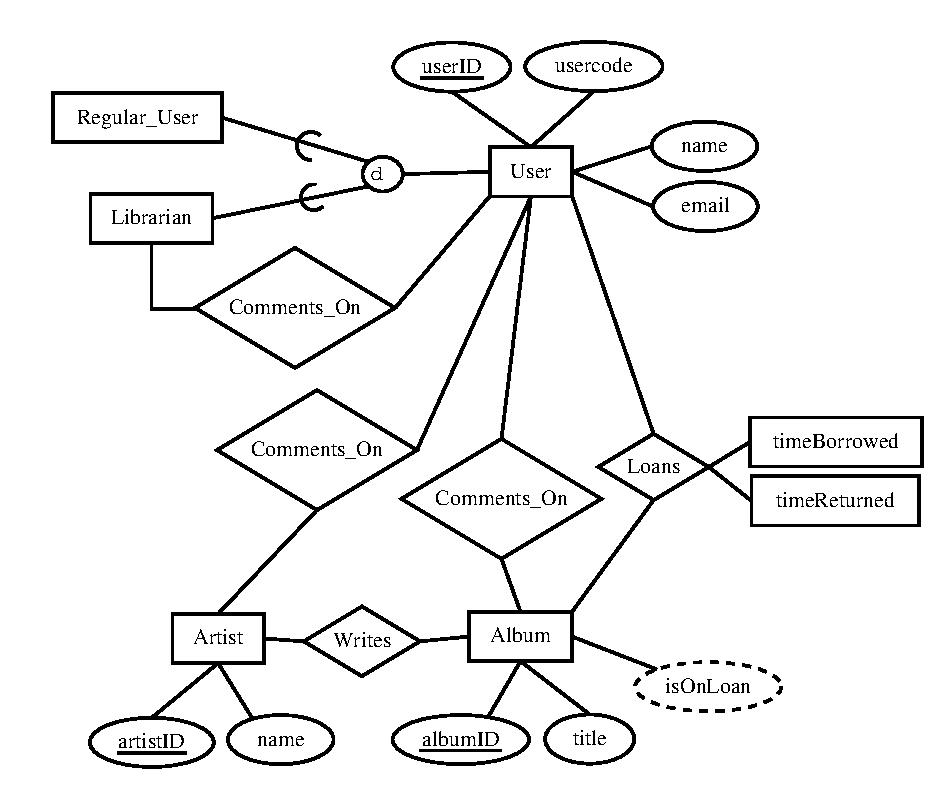
\epsfig{file=ER-Diagram.pdf}
\caption{A figure showing the basic relationships between different entities in the database.}
\label{Fig1}
\end{center}
\end{figure}
%put the ER diagram hereish
\section{Data Structures}
There are many different data structures used to store data within the MusicLib program. Typically for each type of entity that is stored in the database there is one structure associated with holding the data, it is known as a \verb|node|. For example, to hold information about a loan, a \verb|loanNode| is used.
Each type of node is stored in a linked list with other nodes of its type. This section will go through the various nodes and mention the different fields within each one. See Figure \ref{Fig1} for more details.
\subsection{Generic Node Information}
Each Node has a Unique ID value, this is dynamically allocated to it upon creation and remains with it until the database is erased. All nodes  also contain a link to the next node of the same type, as data is accessed and stored within a linked list structure. 
\subsection{Artist, Album and User Nodes}
\begin{description}
\item[artistNode]  contains only one other field storing the name of the artist.
\item[albumNode] contains the title of the album as a String, and the ID of the album's composer.
\item[userNode] contains the user's name, usercode and email address as Strings of characters. Also this structure contains a boolean value which is set to \verb|true| if the user is a librarian or false if they are a standard user.
\end{description}
\subsection{Comment and Loan Nodes}
\begin{description}
\item[userCommentNode] contains a comment about a user, the ID number of the user who wrote the comment and the Id of the user that the comment refers to.
\item[albumCommentNode] contains a comment about an album, the ID of the album that it refers to, and the ID of user who wrote it.
\item[artistCommentNode] contains a comment about an artist, the ID number of the user that wrote the comment and the ID of the artist that the comment refers to.
\item[loanNode] contains the ID of that album that this loan refers to, and the ID of the user who initiated the loan. It also has fields which record the time that the loan was taken out and returned, and finally a boolean value representing whether or not the album has been returned to the library.
\end{description}


\section{Database Layer}
Data within the database is stored to disk as [value]\%[value]\%[value]. The \% character is used as a delimiter between different data objects. This Section will explain the purpose of each `.c' file within the database and what each function achieves.
\subsection{add.c}
This file is responsible for adding to the database. All add functions check fields for invalid input by calling the \verb|checkString| method before performing their intended task. Also each add function checks that the current data does not already exist in the database before adding, so there should never be two of the same entity in the database. At the end of each add function there is a call to the corresponding \emph{save} function described in \verb|save.c|.

\subsubsection*{getctime()}
 This function is a wrapper function for the \verb|getTimeOfDay()| function in \verb|sys/time.h|, it returns the current time of day based on the number of seconds since the Linux epoch 01/01/1970. It is used to record the dates and times of loans within the library.

\subsubsection*{checkString()}
 The checkString function takes in a string and makes sure that it is not null, that it does not begin with a space,  and does not contain any \% characters as these are bad for the database.

\subsubsection*{addUser()}
This function takes in string values for the User's usercode, the User's name, the User's email address, and whether or not the user is a librarian.  These values are mapped to a ``userNode'' and then memory is allocated for each field using \verb|malloc (3)|. This new information is then saved to disk using the \verb|saveUser| function.

\subsubsection*{addAlbum()}
Similar to the addUser, this method allocates the memory for a new Album, and uses the title and artistID passed to it to create a new album in the database. 

\subsubsection*{addArtist()}
This function takes in the name of the new artist, it is given an artist ID using the \verb|_nextArtistID| value, and then memory is allocated for the information using \verb|malloc (3)|.

\subsubsection*{addUserComment()}
This Function is called when a librarian writes a comment about a user. It takes in three different arguments; the \verb|userID| of the user this comment is about, the \verb|owner| or author of the comment, and finally the comment \verb|body| which is the comment itself. Checks are made to make sure the users exist, and then memory is allocated for a new comment struct. The fields are copied to the struct and then it is given an ID field.

\subsubsection*{addAlbumComment()}
This function is essentially the same as the \verb|addUserComment| except that the comment is about an Album. Instead of having a \verb|userID| it is passed an \verb|albumID| to show what album it is about.

\subsubsection*{addArtistComment()}
Again this method closely resembles the addUserComment, it takes in the \verb|artistID| of the artist it is about, the \verb|owner| that wrote it, and the comment \verb|body| itself. These are copied to a \verb|commentNode|.

\subsubsection*{addLoan()}
This function creates a new loan object, meaning that a user wants to borrow an album from the library. The arguments for this are the \verb|userID| of the borrowing user, and the \verb|albumID| of the borrowed album. Both these are checked for validity and then \verb|getctime| is called to record the time that the album was borrowed.

\subsubsection*{addLoanReturned()}
This function is complimentary to the addLoan function, it takes a \verb|loanID| as an argument, checks that it exists and then sets the loan as returned using the set \verb|setLoanReturned| function. Then the return itself is written as information to disk for future reference.

\subsection{get.c}
This file contains all the get functions for the library. Also it has a function to convert special characters to their corresponding html entities.

\subsubsection*{htmlEscape()}
This is the function that converts text values to their proper html syntax, values that are converted are \verb| & `` < > |. Various C functions are used in this process including \verb|malloc (3)|, \verb|strncpy (3)|, \verb|strlen(3)|. Also the function \verb|replaceChar| is used. This is explained in the next section. This function is called every time an item of information is requested from the database, making each displayable by the cgi function calls.

%\subsubsection*{replaceChar()}
%This is the main working part of the \verb|htmlEscape| function. It takes as arguments; the \verb|data| to be searched through, the character to be replaced (\verb|replacee|) and the html string to replace it with (\verb|replacement|).The function then searches through the \verb|data| replacing all instances of the \verb|replacee| character with the \verb|replacement| string.

\subsubsection{User Functions}
\begin{description}
\item[getUser()] returns a user from the database with the requested \verb|userID|. This function is not accessible outside of the database so outsiders cannot directly access or modify the data in the database. All the other User functions call this one in order to access the database information.
\item[getUserExists] returns true if a user is present in the database
\item[makeUserID()] returns a hash value which is used as a \verb|userID|, calculated from the user's \verb|userCode|.
\item[getUserCode()] returns a \verb|userCode| given a user's ID number.
\item[getUserName()] returns a user's name give their ID Number.
\item[getUserEmail()] returns a user's email address given their ID Number.
\item[isUserLibrarian()] returns true if the selected ID Number represents a librarian.
\item[getUsers()] returns an array of all current users in the database.
\item[getUsersCount()] returns the total number of users in the database.
\item[getUsersByType()] returns an array of all the users in the database who are either Librarians or standard users.
\item[getUsersByTypeCount()] returns the number of Librarians or standard users in the database.
\end{description}

\subsubsection{Album Functions}
\begin{description}
\item[getAlbum()] returns an \verb|albumNode_t| with the specified ID Number. Once again this cannot be accessed from outside the database, for data integrity reasons. All other album functions calls this function to retrieve album information from the database.
\item[getAlbumExists()] return true if an album with the specified ID Number exists.
\item[getAlbumTitle()] returns the title of the album with the specified ID Number.
\item[getAlbumArtist()] returns the artist who made the album with the ID Number specified.
\item[getAlbumCurrentLoan()] returns the current \verb|loanID| if the album selected is on loan.
\item[getAlbums()] returns an array of all the albums currently present in the database.
\item[getAlbumsCount()] returns the total number of albums that are currently in the database.
\end{description}

\subsubsection{Artist Functions}
\begin{description}
\item[getArtist()] returns an artist from the database, if the correct artist ID is supplied. All other artist functions call this function.
\item[getArtistExists()] returns true if an artist with the given ID is present in the database.
\item[getArtistName()] returns the name of the artist with the given ID.
\item[getArtists()] returns an array of all the artists currently in the database.
\item[getArtistsCount()] returns the number of artists currently present in the database.
\item[getArtistAlbums()] returns an array of \verb|albumID|'s of albums that this artist has composed.
\item[getArtistAlbumsCount()] returns the number of albums this artist has composed.
\end{description}

\subsubsection{User Comment Functions}
\begin{description}
\item[getUserComment()] returns a \verb|userCommentNode| with the idNumber that is supplied as an argument. 
\item[getUserCommentExists()] returns true if a user comment with the given id exists in the database.
\item[getUserCommentUser()] returns the \verb|userID| of the user that the comment is about.
\item[getUserCommentOwner()] returns the \verb|userID| of the user that made the user comment.
\item[getUserCommentBody()] returns the  user comment that is represented by the given id Number.
\item[getUserCommentsByUser()] returns an array of all user comments made by a user with the supplied ID Number.
\item[getUserCommentsByUserCount()] returns the total number of user comments made by the specified user.
\item[getUserCommentsForUser()] returns an array of all the user comments made about a specific user
\item[getUserCommentsForUserCount()] returns the number of user comments made about the specified user.
\end{description}

\subsubsection{Album Comment Functions}
\begin{description}
\item[getAlbumComment()] returns an \verb|albumCommentNode| with the idNumber that is supplied as an argument. 
\item[getAlbumCommentExists()] returns true if an album comment with the given id exists in the database.
\item[getAlbumCommentAlbum()] returns the \verb|albumID| of the album that the comment is about.
\item[getAlbumCommentOwner()] returns the \verb|userID| of the user that made the album comment.
\item[getAlbumCommentBody()] returns the  album comment that is represented by the given id Number.
\item[getAlbumCommentsByUser()] returns an array of all album comments made by a user with the supplied ID Number.
\item[getAlbumCommentsByUserCount()] returns the total number of album comments made by the specified user.
\item[getAlbumCommentsForAlbum()] returns an array of all the album comments made about a specific album.
\item[getAlbumCommentsForAlbumCount()] returns the number of album comments made about the specified album.
\end{description}

\subsubsection{Artist Comment Functions}
\begin{description}
\item[getArtistComment()] returns an \verb|artistCommentNode| with the idNumber that is supplied as an argument. 
\item[getArtistCommentExists()] returns true if an artist comment with the given id exists in the database.
\item[getArtistCommentArtist()] returns the \verb|artistID| of the artist that the comment is about.
\item[getArtistCommentOwner()] returns the \verb|userID| of the user that made the artist comment.
\item[getArtistCommentBody()] returns the artist comment that is represented by the given id Number.
\item[getArtistCommentsByUser()] returns an array of all artist comments made by a user with the supplied ID Number.
\item[getArtistCommentsByUserCount()] returns the total number of artist comments made by the specified user.
\item[getArtistCommentsForArtist()] returns an array of all the artist comments made about a specific artist.
\item[getArtistCommentsForArtistCount()] returns the number of artist comments made about the specified artist.
\end{description}

\subsubsection{Loan Functions}
\begin{description}
\item[getLoanExists()] returns true if a loan with the given id exists in the database.
\item[getLoanUser()] returns the \verb|userID| of the user that the album is/was loaned to.
\item[getLoanAlbum()] returns the \verb|albumID| of the album that is/was loaned out.
\item[getLoanTimeIn()] returns the time that the loan started.
\item[getLoanTimeOut()] returns the time that the album was returned 
\item[isLoanReturned()] returns true if the album that the loan refers to has been returned.
\item[getLoansByUser()] returns either the loans that have been returned by the specified user, or the loans for albums that have not been returned by the user..
\item[getLoansByUserCount()] returns the number of returned or unreturned loans by the specific user.
\item[getLoansByAlbum()] returns an array of returned or unreturned loans relating to the \verb|albumID| specified. 
\item[getLoansByAlbumCount()] returns the number of returned or unreturned loans relating to the album.
\item[setLoanReturned()] marks the selected loan as returned, and supplies the time that it was returned at.
\end{description}

\subsection{globals.h}
This header file contains 3 different sections;
\begin{description}
\item[Definintions] of the different data file names that are used by the database.
\item[Pointers] to the first node in each of the linked lists used to store every different entity in the database.
\item[ID numbers] for each entity, these are incremented after a new object is added of that entity type.
\end{description}

\subsection{load.c}
This file is used when the program is fist initialized, it loads all the information currently stored in the database, into system memory, using the following methods;

\subsubsection*{loadDatabase()}
This is the main function of this file. It sets all the first variables to Null
and then sequentially calls the other methods in this file, loading and checking each different entity.

\subsubsection*{loadNextID()}
This function loads up the ID's for the various entities within the database, using the file pointed to by \verb|NEXTID_FILE_NAME|

\subsubsection*{loadAllUsers()}
Similar to the \verb|loadNextID| this function loads all artists stored in the database into memory to be accessed by the cgi layer.

\subsubsection*{loadAllAlbums()}
This function loads all the albums from the data files into the current working application.

\subsubsection*{loadAllArtists()}
This function loads all the artists from the database files into the current working application.

\subsubsection*{loadAllLoans()}
\label{loan}
This function retrieves all loan information from the database to be accessed and modified by the cgi application.

\subsubsection*{loadAllLoansReturned()}
This function does exactly the same as \verb|loadAllLoans| except it is for returned loans.

\subsubsection*{Comment loading}
These methods all work similarly to load the different types of comments from the database into working memory.
\begin{itemize}
\item{loadArtistComments()}
\item{loadAlbumComments()}
\item{loadUserComments()}
\end{itemize}

\subsection{read\_line.c}
This file consists of one function that takes in a file and returns the first line of the file as an array of chars.

\subsection{save.c}
This file contains functions to save the various entities within the MusicLib program from system memory to disk.

\subsubsection*{saveNextID}
This function saves all the \verb|nextID|'s to file. Next ID's are the unique id value for each different entity that will be allocated if a new entity of that type is added to the database.

\subsubsection*{Other Save Functions}
All of the following functions write the information they are passed to the appropriate data file in the database.
\begin{itemize}
\item{saveUser}
\item{saveAlbum}
\item{saveArtist}
\item{saveUserComment}
\item{saveAlbumComment}
\item{saveArtistComment}
\item{saveLoan}
\item{saveLoanReturned}
\end{itemize}

\subsection{save.h}
This file provides the function definitions for all the save functions within \verb|save.c|.

\subsection{structs.h}
This file contains definitions for all the structures used within the database to store and retrieve data. Every different entity has a struct related to it,a nd this is where the definitions for these can be found. See the ``Data Structures'' section for more details.

\section{The CGI Layer}
This layer provides the user interface via the use of html forms. It also makes calls to the various database functions depending on what is required by the user.

\subsection{album.c}
This file is responsible for processing the any album requests by the user. These are represented within the code as the \verb|func| variable. The default function of this file is to view the albums in the database. The functions within are described as follows;
\begin{description}
\item[printAlbum()] The initial calling function that initialises the others depending on the request.
\item[doAddAlbum()]Performs basic checks on user and the current request and then calls the \verb|processAddForm| to create a new \verb|albumID|.
\item[doViewAlbum()]Calls the \verb|printAllAlbums| function by default, unless a specific album is requested, then it calls \verb|printSpecificAlbum|.
\item[processAddForm()] This effectively adds the album to the database and returns a message showing either error or success.
\item[printAddForm()] This function outputs to cgi, the html form that the user sees when wanting to add an album.
\item[printAllAlbums()]
Outputs to cgi a list of all the albums currently stored in the database.
\item[printSpecificAlbum()]
Same as \verb|printAllAlbums| except only outputs a single album specified by the user.
\end{description}
These functions are mirrored in most of the other files so many of them will point back here for information. For example in artist.c the first function is \verb|printArtist| which is virtually equivalent to the \verb|printAlbum| function except that it refers to artists not albums. 

\subsection{albumcomment.c}
The first five functions in this file are parallel with those explained in the help for album.c. The following two functions I will explain because they differ slightly.
\begin{description}
\item[printAllAlbumCommentsByUser()]
This function outputs to cgi all the comments written by the specified user about the specified album.
\item[printAllAlbumCommentsForAlbum()]
This function outputs to cgi all the comments written about the album specified by the user.
\end{description}

\subsection{artist.c}
This file is very similar to album.c as is uses the same basic functions to output to cgi, see the album.c help file for more details. 

\subsection{artistcomment.c}
See the help for albumcomment.c as all functions are equivalent with this file, except that this file refers to artists not albums.

\subsection{cgic.c}
This is the standard C library of functions that support the development of web based applications.

\subsection{cgic.h}
This is the standard header file which needs to be included to use the cgic.c library of functions.

\subsection{contact.c}
This file outputs to cgi the html code for the ``Contact Us'' page within the MusicLib program.

\subsection{globals.c}
This file contains two functions that are used globally in the cgi layer of the Musiclib program. 
\begin{description}
\item[userLink()] This function prints an extra link to ``User Info'' if the user has the right permissions.
\item[printTime()] This function prints the current time as a string to output.
\end{description}

\subsection{globals.h}
This file defines the global variables and functions that are used within the cgi layer of the MusicLib program.

\subsection{home.c}
This file simply contains one function \verb|printHome|, this outputs to cgi the details for the homepage of the MusicLib program.

\subsection{loan.c}
Some functions within this file are similar to those explained in the album.c help section, those that are not are explained below;
\begin{description}
\item[doReturnLoan()] This function calls the \verb|processReturnForm| function and outputs whether or not it is successful.
\item[processReturnForm()] This function calls the \verb|addLoanReturned| function which means that the album specified has been returned. It either returns a success or outputs an error message if something goes wrong.
\item[doViewLoan] This function outputs to cgi a page showing all the loans relating to a specific album, if the user has permission to view them.

\item[Printing Specific Loans] The following methods output to cgi, the html code for showing specific types of loans. The loans can either be viewed by user, of which all, current, and previous loans can be shown, or Album where the same is true.
\begin{itemize}
\item{printAllLoansByUser()}
\item{printCurrentLoansByUser()}
\item{printPreviousLoansByUser()}
\item{printAllLoansByAlbum()}
\item{printCurrentLoansByAlbum()}
\item{printPreviousLoansByAlbum()}
\end{itemize}
\end{description}

\subsection{login.c}
The function within this file \verb|printLogin| simply outputs the html code for the login page to cgi when it is called.

\subsection{main.c}
This is the file that controls the web interface using many of the other files in it's directory. It consists of the following functions;
\begin{description}
\item[cgiMain()] This function calls the functions in order that produce the html code for all web pages within the MusicLib program.
\item[theRealWork()] This function deals with login issues and outputs the main starting web page of the MusicLib application, also it outputs the generic header and footer and links for all the pages within the library.
\item[printLinks()] This function outputs the html code for the table of links that are constantly available to users of the MusicLib program. Note that if a user is a librarian, more links are printed.
\item[printHeader()] Similar to \verb|printLinks| this function outputs the \emph{``team44''} header that is used for every page within the library.
\item[printFooter()] This does the same as \verb|printHeader| but instead outputs the html footer that is used on every page within the library.
\end{description}

\subsection{user.c}
This file is very similar to the album.c, see that help file for more details.

The \verb|printAllUsersByType| function does no have an equivalent in album.c, all this method does is output to cgi either all librarians or all standard users depending on the program request.
\subsection{usercomment.c}
This file mirrors albumcomment.c so explanations of all the functions can be found there except the \verb|doShowUserComment| function which is explained below;

This function outputs to cgi, a page with links to all comments that the selected user has made about any other entity. The most common use of this function is when the ``My Comments'' link is clicked within the browser.

\section{Shared Files}
There are two header files and one \verb|.c| file that both the cgi layer and the database use. These files are located within the the ``shared'' directory. They are described below.
\subsection{lib.h}
This file contains method headers for all the methods in the database layer. The cgi layer uses this to know which methods can be called from the database layer.
\subsection{defines.h}
This file contains all the universal error codes and data length restrictions for different fields. 
\subsection{shared.c}
This file contains some string manipulation functions these are defined below:
\begin{description}
\item[toLowerCase()] This function calls \verb|replaceCharWithChar| for each uppercase letter to replace it with the lowercase equivalent. Thus it returns a string of lowercase characters.
\item[replaceCharWithChar] This method takes in a string, and two characters, the one to be replaced (\verb|replacee|) and the one to replace it with (\verb|replacement|), it then loops through the input string and swaps each replacee character with its replacement.
\item[replaceCharWithString] Similar to \verb|replaceCharWithChar| this method takes in an input string, a character to be replaced and a string to replace it with. It loops through the input string and replaces each instance of the replacee character with the replacement string.


\end{description}
\end{document}
